% Adjust these for the path of the theme and its graphics, relative to this file
%\usepackage{beamerthemeFalmouthGamesAcademy}
\usepackage{../../beamerthemeFalmouthGamesAcademy}
\usepackage{multimedia}
\graphicspath{ {../../} }

% Default language for code listings
\lstset{language=C++,
        morekeywords={each,in,nullptr}
}

% For strikethrough effect
\usepackage[normalem]{ulem}
\usepackage{wasysym}

\usepackage{pdfpages}

% http://www.texample.net/tikz/examples/state-machine/
\usetikzlibrary{arrows,automata}

\newcommand{\modulecode}{COMP260}\newcommand{\moduletitle}{Distributed Systems}\newcommand{\sessionnumber}{5}

\begin{document}
\title{\sessionnumber: Mathematics for graphics}
\subtitle{\modulecode: \moduletitle}

\frame{\titlepage} 

\begin{frame}
	\frametitle{Learning outcomes}
	\begin{itemize}
		\item Outcome 1
		\item Outcome 2
		\item Outcome 3
	\end{itemize}
\end{frame}

\part{Vectors}
\frame{\partpage}

\begin{frame}{Vectors}
	\begin{columns}
		\begin{column}{0.48\textwidth}
			\pause A vector has \textbf{components}
			\pause 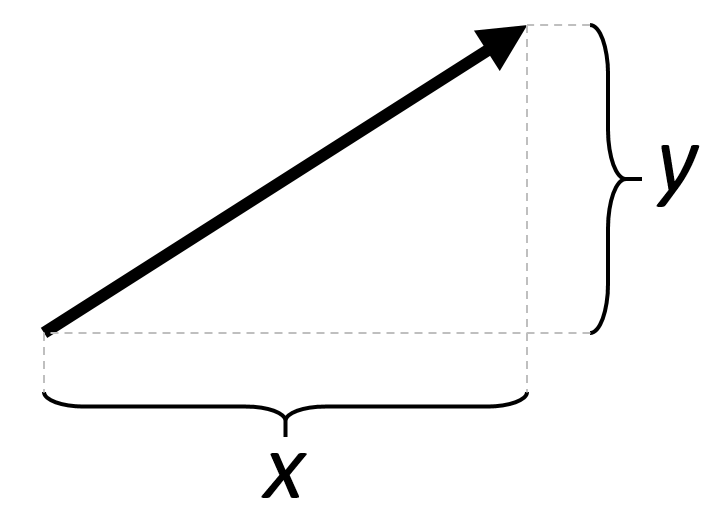
\includegraphics[width=\textwidth]{vector_components}
		\end{column}
		\begin{column}{0.48\textwidth}
			\pause A vector also has \textbf{direction} and \textbf{magnitude} (or \textbf{length})
			\pause 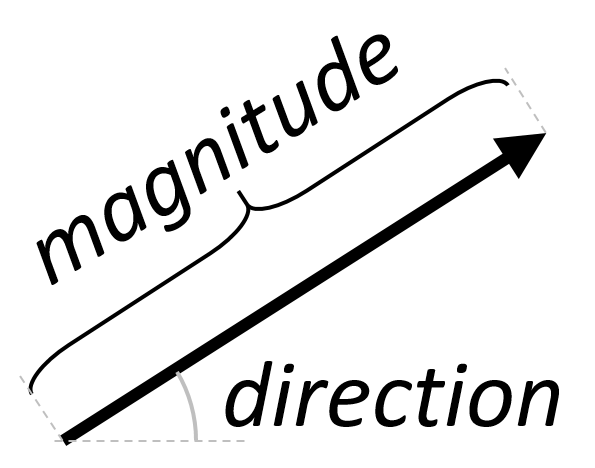
\includegraphics[width=\textwidth]{vector_polar}
		\end{column}
	\end{columns}
	\pause The \textbf{origin} is the point represented by the vector $(0, 0, \dots)$
\end{frame}

\begin{frame}{Radians}
	\begin{itemize}
		\pause\item We often measure angles in \textbf{radians}
		\pause\item $\pi = 3.14159\dots$ 
		\pause\item $\pi \text{ radians} = 180 \text{ degrees} = \text{half a circle}$ 
		\pause\item $\frac{\pi}{2} \text{ radians} = 90 \text{ degrees} = \text{right angle}$
		\pause\item Careful! Some things in OpenGL work in \textbf{degrees}, others in \textbf{radians}
			(just to confuse you...)
	\end{itemize}
\end{frame}

\begin{frame}{Right hand rule}
	\pause OpenGL uses a \textbf{right-handed coordinate system}
	\pause \begin{center}
		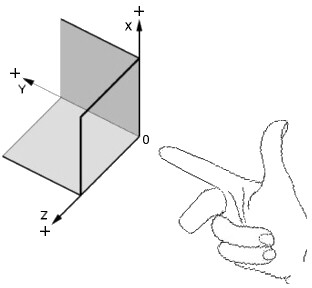
\includegraphics[width=0.3\textwidth]{RightHandRule}
	\end{center}
	\begin{itemize}
		\pause\item The \textbf{$x$-axis} points towards the \textbf{right-hand side} of the screen
		\pause\item The \textbf{$y$-axis} points towards the \textbf{top} of the screen
		\pause\item The \textbf{$z$-axis} points \textbf{out} of the screen
	\end{itemize}
\end{frame}

\begin{frame}{Homogeneous coordinates}
	\begin{itemize}
		\pause\item In 3D graphics, it is useful to represent a \textbf{point in 3D space} as a \textbf{4-dimensional vector}
		\pause\item The extra coordinate is called $w$
		\pause\item Simple explanation: $w$ should always equal $1$ for points in 3D space; having $w$ there makes certain calculations easier
			\begin{itemize}
				\pause\item (Actually, a point $(x,y,z)$ can be represented as a vector $(x \times w, y \times w, z \times w, w)$ for any $w \neq 0$)
			\end{itemize}
		\pause\item In homogeneous coordinates, the origin is $(0, 0, 0, 1)$ not $(0, 0, 0, 0)$!
	\end{itemize}
\end{frame}

\part{Matrices}
\frame{\partpage}

\begin{frame}
	\begin{center}
		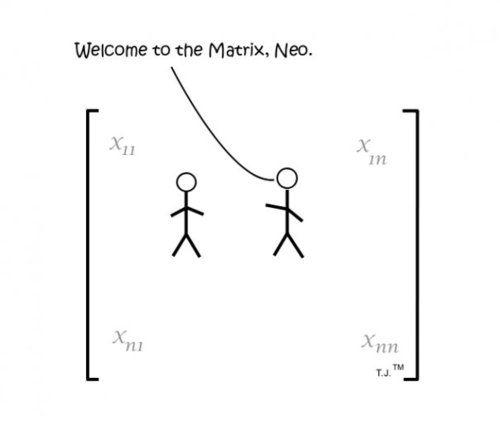
\includegraphics[height=0.8\textheight]{matrixjoke}
	\end{center}
\end{frame}

\begin{frame}{Matrices}
	\begin{itemize}
		\pause\item An $m \times n$ \textbf{matrix} is a rectangular array of numbers, having $m$ rows and $n$ columns
		\pause $$
			\begin{pmatrix}
				3 & 0 & 2.4 \\
				1.7 & -6 & -4.5
			\end{pmatrix}
			\qquad \leftarrow \text{A $2 \times 3$ matrix}
		$$
		\pause\item Note: the plural of \textbf{matrix} is \textbf{matrices}
		\pause\item In computer graphics we mostly work with \textbf{square} matrices (number of rows = number of columns)
	\end{itemize}
\end{frame}

\begin{frame}{Multiplying vectors and matrices}
	\begin{itemize}
		\pause\item Two $n \times n$ matrices can be \textbf{multiplied}, giving a new $n \times n$ matrix
		\pause\item An $n \times n$ matrix and an $n$-vector can be \textbf{multiplied}, giving a new $n$-vector
		\pause\item See \url{https://www.khanacademy.org/math/precalculus/precalc-matrices/multiplying-matrices-by-matrices/v/matrix-multiplication-intro}
		\pause\item (But you don't really need to know how to calculate these manually...)
	\end{itemize}
\end{frame}

\begin{frame}{Commutativity}
	\begin{itemize}
		\pause\item Multiplication of numbers is \textbf{commutative}
			\begin{itemize}
				\pause\item $a \times b = b \times a$
				\pause\item e.g.\ $2 \times 3 = 3 \times 2$
			\end{itemize}
		\pause\item Multiplication of matrices is \textbf{not commutative}
			\begin{itemize}
				\pause\item In general, $A \times B \neq B \times A$
				\pause\item There may be some matrices where $A \times B = B \times A$, but they are the exception
			\end{itemize}
	\end{itemize}
\end{frame}


\part{Transformations in GLM}
\frame{\partpage}

\begin{frame}{Right hand rule}
	\pause OpenGL uses a \textbf{right-handed coordinate system}
	\pause \begin{center}
		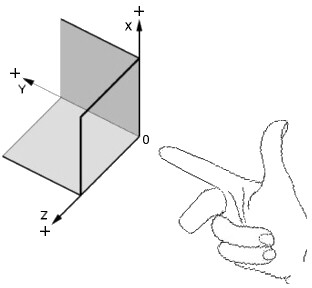
\includegraphics[width=0.3\textwidth]{RightHandRule}
	\end{center}
	\begin{itemize}
		\pause\item The \textbf{$x$-axis} points towards the \textbf{right-hand side} of the screen
		\pause\item The \textbf{$y$-axis} points towards the \textbf{top} of the screen
		\pause\item The \textbf{$z$-axis} points \textbf{out} of the screen
	\end{itemize}
\end{frame}

\begin{frame}{Transformations and matrices}
	\begin{itemize}
		\pause\item A \textbf{transformation} is a \textbf{mathematical function} that \textbf{changes points in space}
		\pause\item E.g.\ shifts them, rotates them, scales them, ...
		\pause\item Many useful transformations can be \textbf{represented} by matrices
		\pause\item Multiplying these matrices together \textbf{combines} the transformations
		\pause\item Multiplying a vector by the matrix \textbf{applies} the transformation
	\end{itemize}
\end{frame}

\begin{frame}[fragile]{GLM}
	\begin{itemize}
		\pause\item We will use the \textbf{GLM} library to do matrix calculations for us
		\pause\item \url{http://glm.g-truc.net/}
		\pause\item GLM aims to mirror GLSL data types (\lstinline{vec4}, \lstinline{mat4} etc) in C++
		\pause\item Lets us perform calculations with vectors and matrices in C++
		\pause\item GLM types can be passed into shaders as uniforms, e.g.
			\begin{lstlisting}
// transformLocation points to a uniform of type mat4
glm::mat4 transform = ...;
glUniformMatrix4fv(transformLocation, 1, GL_FALSE,
				glm::value_ptr(transform));
			\end{lstlisting}
	\end{itemize}
\end{frame}

\begin{frame}[fragile]{Identity}
	\pause The identity transformation does not change anything
	\pause \begin{lstlisting}
// Default constructor for glm::mat4
// creates an identity matrix
glm::mat4 transform;
	\end{lstlisting}
\end{frame}

\begin{frame}[fragile]{Translation}
	\pause Translation shifts all points by the same vector offset
	\pause \begin{lstlisting}
transform = glm::translate(transform,
					glm::vec3(0.3f, 0.5f, 0.0f));
	\end{lstlisting}
\end{frame}

\begin{frame}[fragile]{Scaling}
	\pause Scaling moves all points closer or further from the origin by the same factor
	\pause \begin{lstlisting}
transform = glm::scale(transform,
				glm::vec3(1.2f, 0.5f, 1.0f));
	\end{lstlisting}
\end{frame}

\begin{frame}[fragile]{Rotation}
	\begin{itemize}
		\pause\item How do we represent a rotation in 3 dimensions?
		\pause\item One way is by specifying the \textbf{axis} (as a vector) and the \textbf{angle} (in radians)
		\pause\item Axis always runs through the origin
	\end{itemize}
	\pause \begin{lstlisting}
float angle = glm::pi<float>() * 0.5f;
glm::vec3 axis(0, 0, 1);
transform = glm::rotate(transform, angle, axis);
	\end{lstlisting}
\end{frame}

\begin{frame}[fragile]{Combining transformations}
	\pause \begin{lstlisting}
transform = glm::translate(transform,
					glm::vec3(0.5f, 0.5f, 0.0f));
transform = glm::rotate(transform, angle, axis);
	\end{lstlisting}
	\begin{itemize}
		\pause\item Transformations \textbf{do not commute} in general ---
			changing the order will change the result
		\pause\item The order they are applied is the \textbf{reverse} of what you might think ---
			i.e.\ the above rotates \textbf{then} translates
	\end{itemize}
\end{frame}

\end{document}
